%=================================
\chapter{Exercices récapitulatifs}
%=================================

	La plupart des exercices qui suivent sont inspirés
	d’anciens examens.
	Ils sont assez conséquents et reprennent
	la plupart des notions vues dans ce cours.

	%=================================	
	\section{AEBBCLRS}
	%=================================

		Le Scrabble est un jeu de lettres, 
		où le but est de former des mots ayant le score le plus élevé possible.
		Pour calculer le score d’un mot, 
		une valeur est associée à chaque lettre de l’alphabet. 
		Par exemple la lettre \texttt{A} vaut 1, \texttt{V} vaut 4, 
		\texttt{J} vaut 8,\dots{}
		Le score d’un mot est la somme de la valeur de ses lettres%
		\footnote{dans le vrai jeu c’est un peu plus compliqué.}.

		Par exemple le score du mot \texttt{JAVA} est $8+1+4+1 = 14$.

		Les joueurs tirent chacun 7 lettres qu’ils placent sur un \emph{chevalet}.
		Le but du jeu est de former des mots à partir des lettres du chevalet et de les placer sur le plateau de jeu.
	
		\subsection*{Valeur des lettres}
	
			\'Ecrire un algorithme, \texttt{valeurLettre}, 
			qui reçoit un caractère et retourne sa valeur. 
			Les valeurs des lettres sont les suivantes: 
			\begin{itemize}
			\item A,E,I,L,N,O,R,S,T,U~: 1 point
			\item D,G,M~: 2 points
			\item B,C,P~: 3 points
			\item F,H,V~: 4 points
			\item J,Q~: 8 points
			\item K,W,X,Y,Z~: 10 points
			\end{itemize}	

			L’algorithme lance une erreur avec un message adéquat 
			si le caractère passé en paramètre n’est pas une lettre majuscule.  
	
		\subsection*{Score d’un mot}
			
			\'Ecrire un algorithme, \texttt{scoreMot}, 
			qui reçoit une chaîne de caractères, 
			\texttt{mot}, et retourne la valeur de ce mot, c’est-à-dire la somme de la valeur de chacune de ses lettres.
	
			\underline{Exemple}: si l’algorithme reçoit le mot \texttt{JAVA}, il retourne 14 (=8+1+4+1).
	
		\subsection*{Mot possible}
	
			\'Ecrire un algorithme, \texttt{motPossible}, qui reçoit un tableau de caractères, 
			\texttt{chevalet}, et une chaîne de caractères, 
			\texttt{mot}, et retourne vrai si les lettres du chevalet permettent d’obtenir le mot donné, et retourne faux dans le cas contraire. 
	
	
			\underline{Exemple}: si l’algorithme reçoit le tableau \texttt{[A, O, V, G, G, J, L]} 
			et le mot \texttt{"ALGO"}, l’algorithme retourne vrai. 
			Par contre si le mot donné est \texttt{"JAVA"}, 
			alors l’algorithme retourne faux car la lettre \texttt{A} n’apparait pas 2 fois dans le chevalet.
	
	
			\underline{Aide}~: Une solution possible est de faire une copie du chevalet 
			et pour chaque lettre du mot de vérifier que la lettre s’y trouve, 
			si elle s’y trouve de la remplacer par un symbole (par exemple un '-').
			Pour cela on définit un algorithme \texttt{copieChevalet} 
			permettant de copier un chevalet et un algorithme \texttt{indiceLettre} 
			permettant de connaître l’indice d’une lettre dans un chevalet 
			(cet algorithme retourne -1 si la lettre ne s’y trouve pas). 
	
		\subsection*{Meilleur mot}
	
			\'Ecrire un algorithme, \texttt{meilleurMot}, qui reçoit~:
			\begin{itemize}
			\item un tableau de caractères, \texttt{chevalet}, qui contient les lettres disponibles pour former un mot~;
			\item un tableau de chaînes de caractères, \texttt{dico}, qui contient par exemple tous les mots du dictionnaire.
			\end{itemize}
			L’algorithme retourne le mot du dictionnaire que l’on peut obtenir avec les lettres du chevalet 
			et qui a le score le plus élevé. 
			Si aucun mot n’est possible avec le chevalet, l’algorithme retourne un mot vide \texttt{""}.
	
	%=================================	
	\section{Serpents et échelles}
	%=================================

		Serpents et échelles est un jeu de société
		populaire, se jouant à plusieurs, consistant à déplacer les jetons sur un
		tableau de cases avec un dé en essayant de monter les échelles et en évitant
		de trébucher sur les serpents.	
	
		Pour l’histoire, le jeu peut être perçu comme une représentation d’un chemin
		spirituel que les humains prennent pour atteindre le ciel. Avec des bons
		gestes, le chemin est raccourci (ce que symbolisent les échelles), tandis
		qu’avec de mauvais gestes, le chemin est allongé (d’où vient le symbolisme des
		serpents).
		\begin{flushright}
			Extrait de Wikipedia.		
		\end{flushright}
		
		\subsection*{Représentation du chemin}
		
			Nous représenterons le chemin par un tableau d’entiers. 
			Chaque case du tableau contiendra une valeur~:
			\begin{itemize}
				\item positive pour représenter une échelle et permettre d’avancer plus vite~;
				\item négative pour représenter le serpent et ralentir (voire reculer).
			\end{itemize}
	
		\subsection*{Règles du jeu}
		
			Pour jouer, le joueur qui a la main lance le dé et avance de la valeur
			indiquée par le dé. À partir de cette nouvelle position, il vérifie la
			valeur de la case sur laquelle il se trouve pour continuer à avancer ou au
			contraire reculer. Si la valeur est positive, il avance et si elle est
			négative, il recule de la valeur contenue dans la case.
		
			Si la case est déjà occupée, le joueur se placera sur la case suivante. 
		
			Le joueur passe la main au joueur suivant. 
			
			\textbf{Exemple.} Le joueur se trouvant à la position 3 lance le dé. Il
			obtient la valeur 4. Il avance de 4 cases et se retrouve sur la case en
			position 7 qui contient la valeur 2. Il avance encore de 2 cases … et
			termine donc son tour en position 9. Il passe alors la main au joueur suivant.
		
			\begin{center}
				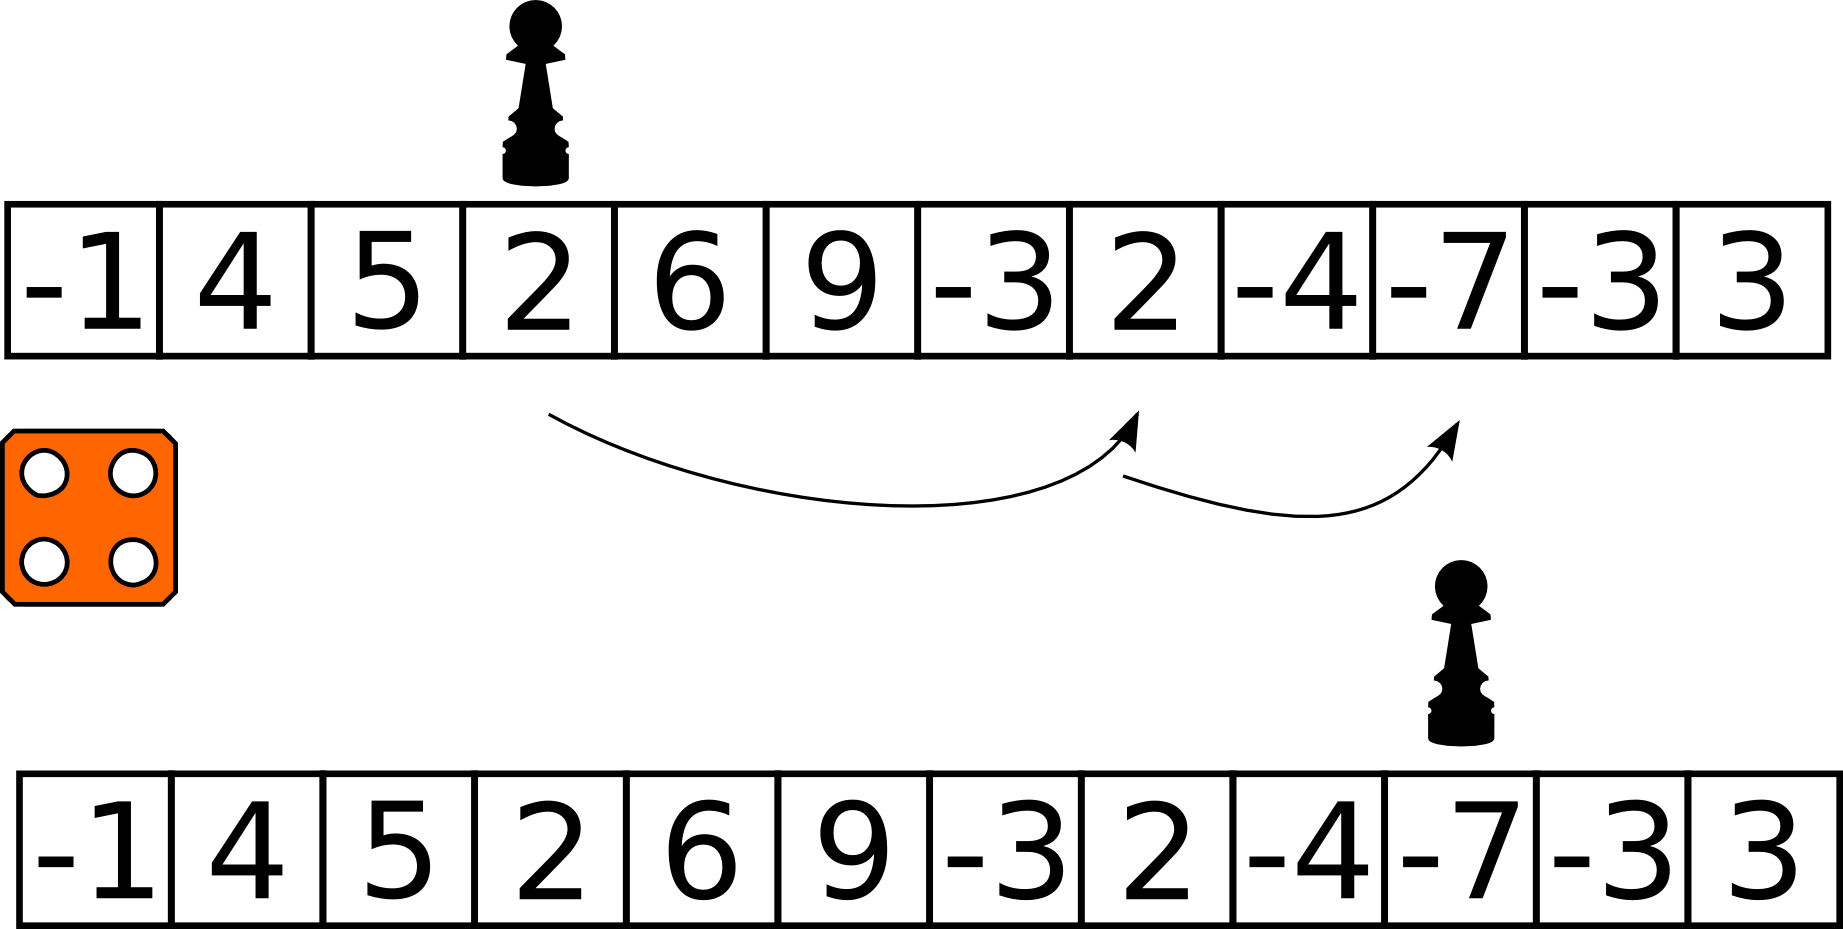
\includegraphics[width=280px]{image/snake-1}
			\end{center}
			
			Le premier joueur à atteindre ou dépasser la dernière case a gagné. Nous supposerons que
			cette dernière case est en position 42. Nous supposons également que la première et la dernière case n’ont ni échelle ni serpent (valeur nulle).
	
		\subsection*{Positions des joueurs}
		
			Les positions des joueurs seront mémorisées dans un tableau d’entiers. 
			Toutes les cases de ce tableau sont initialisées à 0. 
		
			Le plateau de jeu, un tableau d’entiers s’appellera \textbf{chemin}. 
		
			Le tableau d’entiers contenant la position courante des joueurs s’appellera
			\textbf{positionsJoueurs}. 
		
			S’il y a 4 joueurs, le tableau \textit{positionsJoueurs} contient 
			[2,5,1,7] alors~:
			\begin{itemize}
				\item le joueur 0 est en position 2 sur le chemin~;
				\item le joueur 1 est en position 5 sur le chemin~;
				\item le joueur 2 est en position 1 sur le chemin~;
				\item le joueur 3 est en position 7 sur le chemin~;
			\end{itemize}
				
		\subsection*{Le premier jour, initialiser le chemin}
		
			Écrivez un algorithme 
			\begin{LDA}
			\Entete{créerChemin}{\Par{n\In}{entier}}{\Array{n}{entier}}
			\end{LDA}
			
			Cet algorithme \textit{créerChemin} créera un tableau d’entiers
			dont les valeurs seront des valeurs aléatoires 
			comprises strictement entre -10 et 10 (inclus). 
		
			Nous supposons que l’entier $n$ est un naturel strictement supérieur à 0.
			Vous ne devez pas le vérifier. 
	
		\subsection*{Qui est en tête~?}
	
			Écrivez un algorithme 
		
			\begin{LDA}
			\Entete{enPremièrePosition}{\Par{positionsJoueurs\In}{\Array{m}{entier}}}{entier}
			\end{LDA}
			
			Cet algorithme retourne le numéro du joueur en tête de la course. 
			Il recherche donc le maximum dans le tableau passé en
			argument et retourne l’indice de ce maximum. 
	
		\subsection*{Jouer un tour de jeu}
	
			Cet algorithme permettra de jouer un tour de jeu pour un joueur donné. Jouer un
			tour de jeu consiste à le faire avancer ou reculer (c’est-à-dire changer sa
			position) du bon nombre de cases. 
	
			\begin{LDA}
			\Entete{jouer}{
				\Par{chemin\In}{\Array{n}{entier}},
				\Par{positionsJoueurs\InOut}{\Array{m}{entier}},
				\Par{joueurCourrant\In}{entier},
				\Par{valeurDé\In}{entier}
				}{}
			\end{LDA}
		
			Cet algorithme fait changer de position le joueur d’indice
			\textit{joueurCourrant} de la valeur donnée par le dé (\textit{valeurDé}) en
			respectant les règles du jeu. 
		
			Cet algorithme met donc à jour le tableau \textit{positionsJoueurs}. 
		
			Comme le joueur ne peut se placer sur une case déjà occupée, il peut être
			utile d’écrire un module \texttt{estOccupé} précisant si la
			case est libre ou occupée.  
	
	%=================================	
	\section{Les algorithmes en maternelle}
	%=================================

		En maternelle, déjà, les enfants font des algorithmes 
		mais il s’agit d’une chose un peu différente.
		On leur propose un collier\footnote{%
			Par exemple, mais ça peut aussi être une chenille,
			un escargot, une simple suite de cases\dots
		}
		dessiné sur une feuille de papier 
		et ils doivent le colorier en répétant un
		\emph{motif} donné\footnote{%
			Ce qu’ils appellent un \emph{algorithme}.
		}, 
		une séquence précise de couleurs.
		
		Par exemple, on donne ce collier 
		\ \perle{red}-\perle{red}-\perle{green}-\perle{white}-\perle{white}-\perle{white}-\perle{white}-\perle{white}-\perle{white}-\perle{white}\ 
		qui est pré-colorié avec deux perles rouges et une perle verte, c’est le motif.
		\\Le résultat attendu est~:
		\perle{red}-\perle{red}-\perle{green}-\perle{red}-\perle{red}-\perle{green}-\perle{red}-\perle{red}-\perle{green}-\perle{red}.
		
		Comme on peut le constater sur cet exemple,
		un motif peut comporter plusieurs perles de la même couleur
		et, en fin de collier, il est possible qu’on ne puisse
		appliquer qu’une partie du motif.
		
		\textbf{Nous allons representer chaque perle par un caractère
		indiquant sa couleur et un collier comme un tableau de caractères.
		Une perle non coloriée sera indiquée par un point (\Verb_'.'_).}
		
		Par exemple, le collier ci-dessus serait représenté ainsi~:
		
		\begin{center}
		\begin{tabular}{|*{10}{>{\centering\ttfamily\arraybackslash}m{6mm}|}}
		\hline
		'R' & 'R' & 'V' & '.' & '.' & '.' & '.' & '.' & '.' & '.' \\
		\hline
		\end{tabular}
		\end{center}
	
		\subsection*{Créer un collier}
		%-----------------------------------------
		
			Écrivez un algorithme \textbf{créerCollier}
			qui reçoit une taille et crée un collier de cette taille
			où toutes les perles sont non coloriées
			(rappel~: une perle non coloriée est représentée par un point).
			
			On suppose que la taille reçue est bien un entier non négatif.
	
		\subsection*{Créer un motif}
		%-----------------------------------------
		
			Écrivez un algorithme \textbf{créerMotif}
			qui reçoit un collier dont aucune perle n’est coloriée
			et qui colorie les premières en fonction des indications
			de l’utilisateur.
			
			Concrètement,
			l’utilisateur entre les couleurs des perles
			en spécifiant à chaque fois, après,
			s’il y a encore une perle à colorier.
			Dans notre exemple de la première page,
			l’utilisateur entrerait successivement~:
			'R', vrai, 'R', vrai, 'V', faux. 
			
			L’algorithme doit vérifier que l’utilisateur
			ne demande pas à colorier plus de perles
			qu’il n’y en a dans le collier.
	
		\subsection*{Taille du motif}
		%-----------------------------------------
	
			Écrivez un algorithme \textbf{tailleMotif}
			qui reçoit un collier dont seulement les premières perles sont coloriées
			(c’est le motif qu’il faudra suivre)
			et qui donne la taille de ce motif.
			Dans l’exemple de la première page, il faudra retourner la valeur 3.
			Votre algorithme doit générer une erreur si il n’y a pas de motif à suivre.
	
		\subsection*{Suivre un motif}
		%-----------------------------------------
		
			Écrivez un algorithme \textbf{colorier}
			qui reçoit un collier dont seulement les premières perles sont coloriées
			(c’est le motif qu’il faut suivre)
			et qui colorie le reste du collier en suivant ce motif.
			
		\subsection*{Vérifier un collier}
		%-----------------------------------------
		
			Écrivez un algorithme \textbf{vérifier}
			qui reçoit un collier complètement colorié
			et la taille du motif de départ et qui vérifie
			si le collier respecte ce motif.
		
		\subsection*{Trouver le motif}
		%-----------------------------------------
		
			Écrivez un algorithme \textbf{trouverMotif}
			qui reçoit un collier complètement colorié
			et qui détermine la taille du motif.
			C’est la plus petite séquence qui se répète.
			Comme cas extrème, ce pourrait être le collier tout entier.
		
			Aide~: vous avez déjà tout pour que cet exercice soit facile.

